\documentclass[10pt]{report}
\usepackage{fullpage}
\usepackage[T1]{fontenc}
\usepackage{graphicx}
\usepackage{amsmath}
\usepackage{comment}
\usepackage{amssymb}
\usepackage{amsthm}
\usepackage{fancyvrb}
\usepackage{amsfonts}
\usepackage{algorithm}
\usepackage[noend]{algpseudocode}
\usepackage{graphicx}
\usepackage{array}
\usepackage{xltabular}
\usepackage[export]{adjustbox}
\graphicspath{ {./images/} }
\theoremstyle{definition}
\newtheorem{definition}{Definition}
\theoremstyle{plain}
\newtheorem{theorem}{Theorem}
\newtheorem{lemma}{Lemma}
\newtheorem{example}{Example}[section]

\parindent0in
\pagestyle{plain}
\thispagestyle{plain}

%% UPDATE MACRO DEFINITIONS %%
\title{MDL Genetic Algorithm project report}
\author{Rutvij Menavlikar (2019111032) \\ Tejas Chaudhari (2019111013)}

\begin{document}

\begin{titlepage} 
    \maketitle{}
\end{titlepage}

\section*{Overview of the Algorithm}
The structure of our Genetic algorithm is the same as a normal Genetic Algorithm, but we have implemented a custom crossover function rather than a standard crossover function. \\
\begin{figure}[h]
\centering
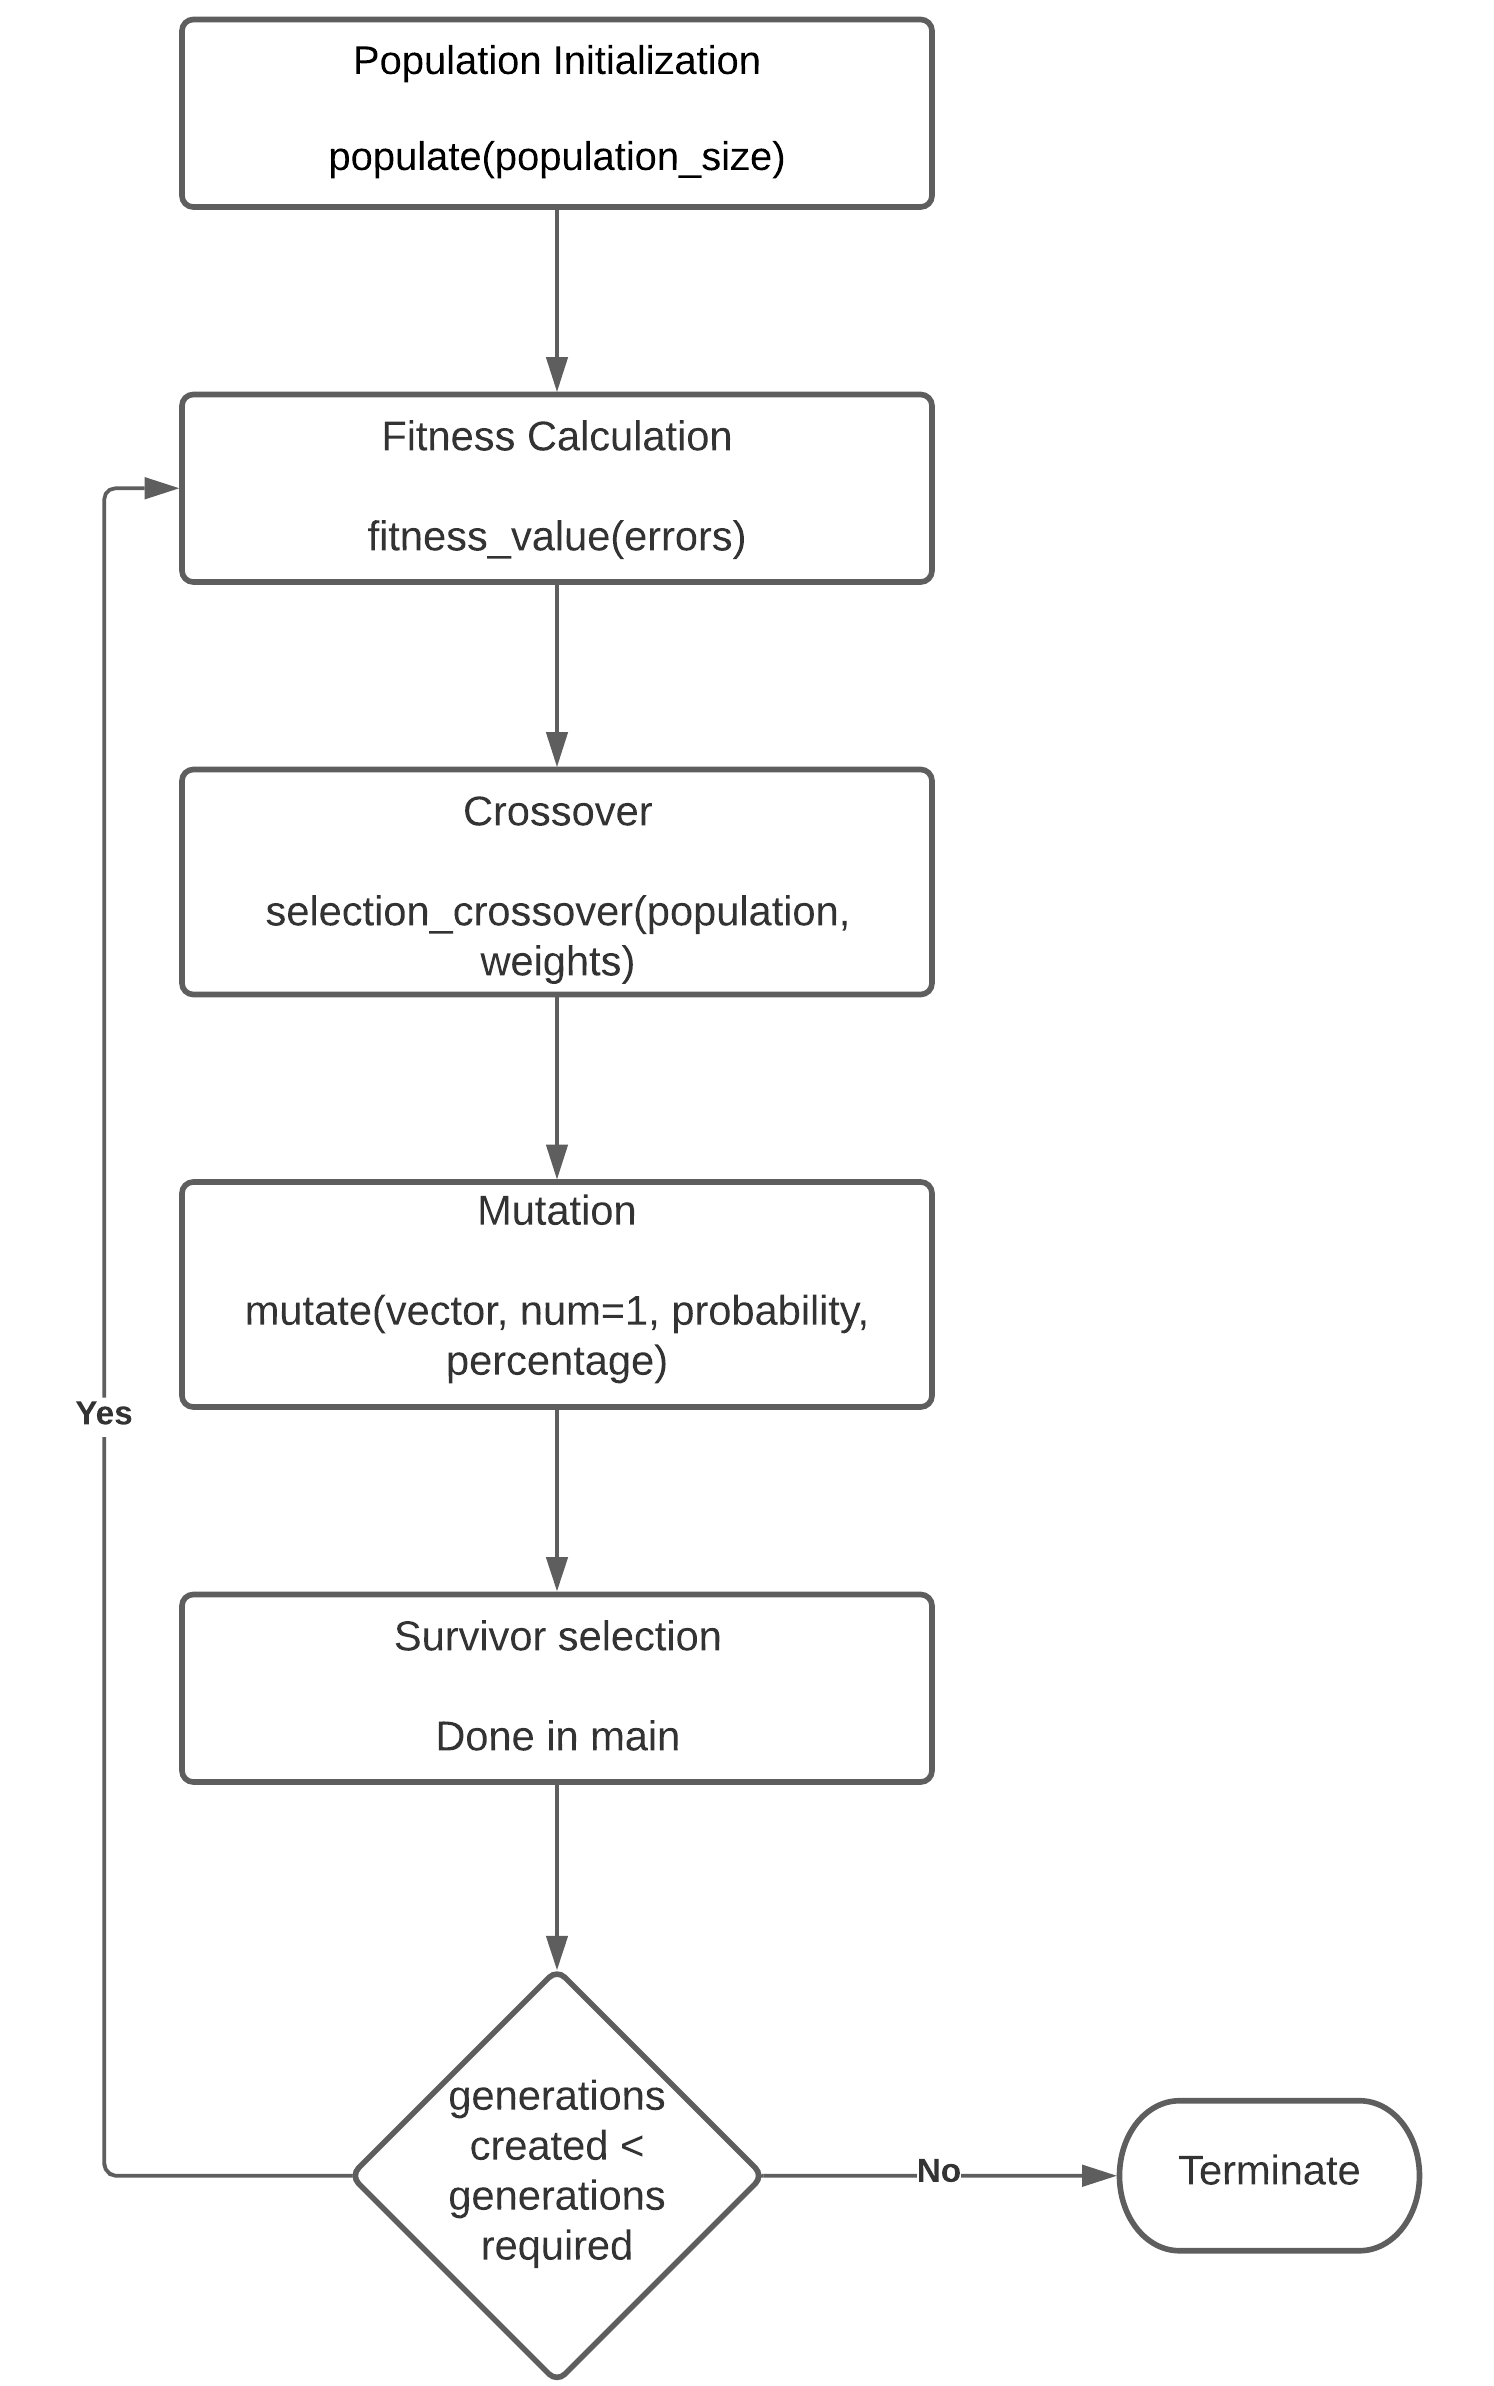
\includegraphics[height=14.9cm]{1.png}
\caption{Flowchart representing the Genetic Algorithm}
\end{figure}
\section*{Iterations}
\begin{figure}[htp]
\centering
% \includegraphics[height=1.0\textwidth]{iteration_diagram.png}
\includegraphics[max size={\textwidth}{\textheight}]{iteration_diagram.jpg}
\caption{Diagram denoting running of algorithm for 3 iterations}
\end{figure}
\pagebreak



\section*{Fitness function}
We have calculated fitness for a vector using the formula: \\ \\
$\frac{1}{\text{|(train\_error x TRAIN\_FACTOR) + (validation\_error x TEST\_FACTOR) + (|train\_error - validation\_error| x DIFF\_FACTOR) |}}$ \\ \\

We are using reciprocal of errors since minimizing errors should maximize fitness. We are also adding the difference term to make sure that we do not overfit our algorithm on either training or validation dataset.

\section*{Crossover function}
We have implemented a custom crossover function. The basic idea it to use uniform crossover for n vectors, where n is randomly chosen. The process is:\\
\begin{center}
 \begin{tabular}{||c | c||} 
 \hline
 n & Probability \\
 \hline\hline
 2 & 35\% \\
 \hline
 3 & 45\% \\
 \hline
 4 & 20\% \\
 \hline
 \hline
\end{tabular}
\end{center}
We have done this since we believe that 2 vectors may leave out some information, 3 vectors contains enough information. and 4 vectors may contain additional unnecessary information. \\

Suppose we select n vectors and label them in alphabetical order starting from a in decreasing order of fitness. Let our final vector be x, then we have defined x to be:
\begin{center}
    For n = 2, $x_i = $\\
    $a_i, 60\%$ \\
    $b_i, 40\%$ \vspace{0.3cm}
    
    For n = 3, $x_i = $\\
    $a_i, 50\%$ \\
    $b_i, 30\%$ \\
    $c_i, 20\%$ \vspace{0.3cm}
    
    For n = 4, $x_i = $\\
    $a_i, 45\%$ \\
    $b_i, 25\%$ \\
    $c_i, 15\%$ \\
    $d_i, 15\%$ \vspace{0.3cm}
\end{center}
Note: \textit{For n = 4, we decided to keep the probability for vectors c and d equal since they probably won't differ much in fitness, but still can help in randomization.}
\pagebreak
   
\section*{Mutations}
We mutate our vector(x) using the following algorithm: \\
For each dimension in x: \\
- Choose to mutate this dimension with probability MUTATION\_PROB \\ \hspace*{0.4cm}
    - If chosen to mutate, check if the weight of current dimension is 0: \\ \hspace*{0.8cm}
        - If weight of current dimension if 0, assign a random value between the given range of weights. \\ \hspace*{0.8cm}
        - If weight of current dimension is not 0, then add a random value between -VAR\_PERCENTAGE of $x_i$ and VAR\_PERCENTAGE of $x_i$ \\ \hspace*{0.8cm}
        - Continue to next dimension \\ \hspace*{0.4cm}
    
    - If chosen not to mutate, continue to next dimension \\

\section*{Hyperparameters}
POPULATION\_SIZE = 10, number of vectors per generation \vspace{0.1cm} \\ 
GENERATIONS = 9, Number of generations to create \vspace{0.1cm} \\
MATING\_POOL\_SIZE = 10, number of vectors considered during crossover vector selection \vspace{0.1cm} \\
MIN = -10, Minimum weight of a dimension \vspace{0.1cm} \\ 
MAX = 10, Maximum weight of a dimension \vspace{0.1cm} \\ 
MUTATION\_PROB = 0.7. Probability that a dimension will be chosen for mutation \vspace{0.1cm} \\
VAR\_PERCENTAGE = 25, max percentage that can be added or subtracted from the dimension during mutation \vspace{0.1cm} \\
ORIGINAL\_ERROR = 381807315968.0, original overfit vector's sum of training set error and validation set error \vspace{0.1cm} \\
BEST\_PARENTS = 3, number of parents which will be passed on to next generation \vspace{0.1cm} \\
TRAIN\_FACTOR = 0.95, multiplied to the training error to increase or decrease its contribution to the fitness value \vspace{0.1cm} \\
TEST\_FACTOR = 1.0, multiplied to the validation error to increase or decrease its contribution to the fitness value \vspace{0.1cm} \\
DIFF\_FACTOR = 1.0, multiplied to the absolute difference of validation error and test error to increase or decrease its contribution to the fitness value \vspace{0.1cm} \\
MIN\_MUTATE = 100, minimum number of times we mutate a vector while creating the initial population from the overfit vector \vspace{0.1cm} \\
MAX\_MUTATE = 1000, maximum number of times we mutate a vector while creating the initial population from the overfit vector \vspace{0.1cm} \\

\section*{Statistics}
\subsection*{Iteration Needed to converge}
Starting from the overfit vector, the code took approximately \textbf{100} generations for the training set MSE to overtake the validation set MSE. \\
But, the fitness function used for these generations did not consider the difference between the errors. \\
It then took approximately \textbf{2000} generations to converge to the final vector.

\subsection*{Number of Restarts}
We restarted training vector \textbf{3} times.
\begin{enumerate}
    \item When we switched from making a completely randomised population, to filling the population with mutated vectors of the overfit vector.
    \item When we realised that our \emph{mutate} function was incorrect. (We were replacing given weight with a random value in the given range for weights.)
    \item When we added a mating pool, and stored previous code run's final generation population and their errors.
\end{enumerate}
For the changes made after these, we retained the generation and created branches of generations, in a way that we could revert back to a population of a generation we know is best. This data is stored in the file named \emph{population.txt}.

\section*{Heuristics used}
1) Directional mutation (failed): \\
Tried to use the best vectors of a population to add a bit of bias to mutations that increase the fitness but we could not determine whether it was helpful or not and all vectors started to converge too rapidly. \\

2) Binary crossover (failed): \\
Tried using binary crossover but the performance decreased when using it. \\

3)  Mutate (failed): \\
For weight of each dimension of the vector, replace it by a random value in the given range for weights. \\

4) Singlepoint crossover (partial success): \\
Used single point crossover in the beginning but it stopped giving better vectors after a certain amount of time. Replaced with Hybrid Crossover \\

5) Hybrid crossover (partial success): \\
This was our intermediate solution in which we used single point crossover with probability 60\% and uniform crossover with probability 40\%. Replaced this with our selection crossover \\

6) Elitism (Used): \\
We are using elitism while forming the new generation \\

7) Population creation (Used): \\
We are mutating the initial overfit vector POPULATION\_SIZE - 1 times to create our initial population if not given. \\

8) selection crossover (Used): \\
Explained in the crossover section \\

\pagebreak
\section*{Train and Validation error}
\begin{center}
% \begin{xltabular}{\textwidth}{|m{1cm}|m{8cm}|m{3cm}|m{3cm}|}
\begin{xltabular}{\textwidth}{
|>{\hsize=.2\hsize}X|
>{\hsize=2.2\hsize}X|
>{\hsize=0.8\hsize}X|
>{\hsize=0.8\hsize}X|
}
    \hline
    \multicolumn{1}{|c}{S. No.} & \multicolumn{1}{|c}{Vector} & \multicolumn{1}{|c}{Training set MSE} & \multicolumn{1}{|c|}{Validation set MSE}\\
    \hline 
    \hline 
    1. & [1.0796526941030586, -8.715162711943131e-19,\newline 3.871354440528529e-06, 1.7653154651736457e-09,\newline -1.2486049836655162, 2.1471529604497616e-18,\newline 5.094795413663314e-21, 2.4044189773090542e-14,\newline 1.0558133124332984e-07, -9.757122653416584e-16,\newline -1.444904845379374e-14] & 85789478076.08893 & 85860947393.53752\\
    \hline
    2. & [0.7418155574643469, -3.4450243325386273e-18,\newline 3.2261440074855244e-06, 3.175351759871859e-09,\newline -1.2486049836655162, 7.17799837783098e-19,\newline 5.0167540463567284e-21, 2.483229218868748e-14,\newline 1.056441508086754e-07, -1.8213786816009663e-15,\newline -1.0019745817707677e-14] & 85952768142.60727 & 86005658803.69467\\
    \hline
    3. & [1.847052262841336, -2.5068768507801048e-18,\newline 4.659740503058584e-06, 2.2800933816946775e-09,\newline -1.2486049836655162, 3.9945130632584965e-19,\newline 6.535555699401268e-21, 2.5784437558132038e-14,\newline 1.056441508086754e-07, -3.0391827416463197e-15,\newline -7.38011537222921e-15] & 86008133144.05466 & 86023162332.26974\\
    \hline
    4. & [2.0780107356915596, -3.992838840428164e-18,\newline 4.516809843168537e-06, 2.8002915027458477e-09,\newline -1.2486049836655162, 2.8818471692097994e-19,\newline 8.129227218592027e-21, 5.215097700409277e-14,\newline 1.056441508086754e-07, -3.300387853578753e-15,\newline -4.8213371071931044e-15] & 86018693956.65129 & 86034879036.24663\\
    \hline
    5. & [2.388702449057477, -4.428532357378065e-18,\newline 3.719949358824128e-06, 2.7070450375210467e-09,\newline -1.2486049836655162, 1.712455798799604e-19,\newline 7.808053560215505e-21, 5.0302136123933467e-14,\newline 1.056441508086754e-07, -1.9898530793314443e-15,\newline -3.9842623013157476e-15] & 86039524180.61018 & 86040999679.32416\\
    \hline
    6. & [2.6818812113350003, -4.314964270135856e-18,\newline 4.057299232887971e-06, 6.826389375060461e-09,\newline -1.2486049836655162, 1.5553402114948158e-19,\newline 1.3314811505159597e-20, 6.85844393372265e-14,\newline 1.056441508086754e-07, -3.2542763496813605e-15,\newline -2.7153269412270014e-15] & 86036286133.70601 & 86045633451.5842\\
    \hline
    7. & [10.0, -9.150504594076882e-18,\newline 5.0533594624717434e-06, 9.84543056488233e-10,\newline -1.2486049836655162, 4.3576463454620555e-20,\newline 8.53887837444912e-21, 1.128015450719615e-13,\newline 1.0563239599063873e-07, -7.908235682492684e-15,\newline -4.671789492731e-15] & 86094693232.60085 & 86024187443.89883\\
    \hline
    8. & [6.721321544621738, -1.1877921234621972e-17,\newline 6.8904241546123365e-06, 5.7470406913645966e-09,\newline -1.2486049836655162, 4.4656815455991816e-20,\newline 4.025632784891203e-21, 1.4104150950287807e-13,\newline 1.0563239599063873e-07, -8.756274436367583e-15,\newline -8.692630883341574e-15] & 86116468204.83037 & 86010770562.37679\\
    \hline
    9. & [6.8844350902206175, -9.794730566767862e-18,\newline 1.828988602880485e-05, 4.855622630975936e-09,\newline -1.2486049836655162, 1.834386010950058e-20,\newline 4.35552545923755e-21, 1.2062971267624513e-13,\newline 1.0574888606925636e-07, -1.5686936339548276e-14,\newline -1.3673296891880275e-14] & 85918806169.71979 & 86163120117.01878\\
    \hline
    10. & [4.184070668290893, -7.850456642755217e-18,\newline 2.6623847537377427e-05, 5.036305913703038e-09,\newline -1.2582264023072198, 1.9616216160068823e-20,\newline 3.7313992965337805e-21, 4.931505123879456e-13,\newline 1.0664583512488755e-07, -8.623342104104946e-15,\newline -1.2760055435313701e-14] & 86220260976.6219 & 86231590827.8452\\
    \hline
\end{xltabular}
\end{center}
After beginning from the training set MSE and validation set MSE of the overfit vector, \textit{(13510723202.57021, 368296581138.17303)}, the vectors generated by our algorithm are better in the following ways:
\begin{itemize}
    \item The training set MSE is larger than that of overfit vector, which indicates that the new vector is no longer overfit on the training set.
    \item The validation set MSE is less than that of overfit vector, which indicates that the new vector performs better than the overfit vector on a data set other than the one it was trained on.
    \item The difference between training set MSE and validation set MSE is much less than that of overfit vector, which indicates that the new vector is standardised on both, training set and validation set, and that it has a good chance to do well on an unseen data set.
\end{itemize}

\pagebreak
\section*{Miscellaneous tricks}
\subsection*{Select Unique Vectors}
While choosing vectors for crossover, we are making sure to select unique vectors using weighted probability.
\begin{figure}[ht]
\centering
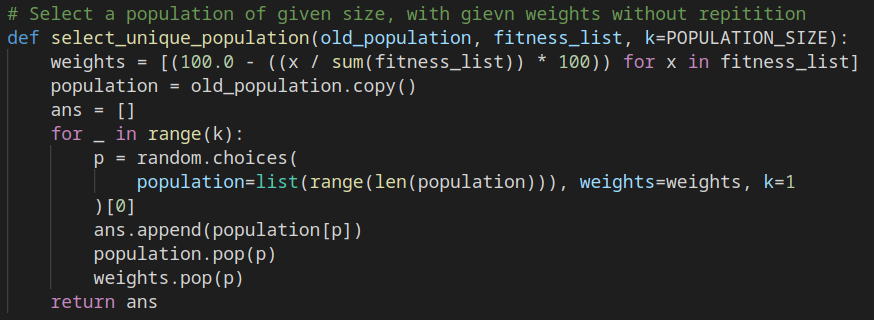
\includegraphics[width=1.0\textwidth]{2.png}
\caption{Function in the code to select k unique vectors from a given population with weighted probability}
\end{figure}


\end{document}